\documentclass[12pt]{report}
\usepackage[margin=2cm]{geometry}
\usepackage{titlesec, sectsty, amsmath, mathtools, graphicx, numprint, titling}
\title{Multistage Predictor for Cellular Network Throughput Prediction}
\author{Killian Nolan}
\date{2023}
\titleformat{\chapter}[display]
{\normalfont\bfseries}{}{0pt}{\fontsize{20}{16}\selectfont}
\newcommand*{\figuretitle}[1]{%
    {\centering%   <--------  will only affect the title because of the grouping (by the
    \textbf{#1}%              braces before \centering and behind \medskip). If you remove
    \par\medskip}%            these braces the whole body of a {figure} env will be centered.
}
\begin{document}
\maketitle
\newgeometry{top=0.9cm, left=2cm}
\chapter{Abstract}
Accurate throughput prediction is an important component of many of today's communication systems such as video streaming or the scheduling of large downloads. Today's world heavily utilizes wireless communication technologies such as 4G and 5G for such applications, however throughput prediction for wireless systems presents a unique challenge for application designers due to the highly dynamic nature of wireless networks. Deep learning based throughput prediction models have previously been recognised as a good approach to tackling this problem due to the high dimensionality and complexity of cellular data. This project aims to expand on these previous works by creating a multi-stage deep learning model. The goal of the multi-stage model is to better accommodate for the imbalanced nature of cellular data and improve upon the deep learning model's ability to generalize.
\chapter{Declaration}
I hereby declare that the contents of this paper and the work surrounding it are my own.
Signed - Killian Nolan.
\chapter{Acknowledgements}
Write them here
\tableofcontents
\chapter{Introduction}
Total mobile network traffic has doubled over the last two years and is expected to increase a by a factor of 4 by the year 2028. This is due to growth in the number of mobile devices as well as the use of 5G mobile networks \cite{Eri22}. Cellular networks are highly dynamic systems. The system conditions are highly variable and depend on various constantly changing factors such as the level of interference, location, line of site etc. Throughput is heavily dependent on the current condition of the network channel and as such can vary dramatically of the course of a few seconds. This presents a challenge for both the network itself, and the mobile devices that leverage the network. The network attempts to balance its available resources between all of its connected users and applications running on the mobile devices require knowledge of the available throughput in order to function correctly. 

A notable use case of throughput prediction on cellular networks relates to video streaming. The vast majority of mobile network traffic is video streaming \cite{Eri22}. Video streaming applications require high network throughput and good consistency in order to deliver the video quality we expect in today's world. Video streaming requires that chunks of the video be downloaded in a timely manner before they are used. The application will dynamically adjust the size of the chunk of the video it attempts to download depending on throughput predictions. For example if the throughput prediction algorithm in use predicts a low download bitrate over the next few seconds the application will schedule the download of a lower quality video chunk as lower quality means less overall data. Failure to adapt to the current network environment may result in buffering or noticeable changes in quality throughout a video for the user. Accurate throughput prediction plays a key role in maintaining the quality of user experience in these applications \cite{raca2019improving}. 

Adoption of currently niche technologies such as AR (augmented reality) and VR (virtual reality) is projected to increase in the near future \cite{Sta22}. These technologies will make heavy use of cellular networks for device mobility and ergonomics. VR and AR devices require low latency and high throughput connections to function optimally. Right now this is achieved by tethering such devices to a network via a physical wire. This limits the potential use cases and adoption of such technologies. 5G can provide the latency and throughput requirements for optimal operation of these technologies allowing them to be used in more mobile devices. As such they stand to benefit from accurate throughput prediction.

Multistage models make use of 2 or more models to solve a given problem. This can be done when the problem can be broken up into smaller pieces which can be solved separately. The models may be linked together sequentially or in parallel depending on how the problem was decomposed. The intuition behind using a multistage approach as opposed to tradition single model approaches is that throughput in a cellular channel is inherently imbalanced. As seen in this paper, typical download throughput levels fall in the ranges above 5Mbps. User experience is disproportionally influenced by low throughput situations such as <5Mbps or <1Mbps as opposed to differences experienced outside these bounds \cite{raca2019improving}. Models trained on smaller sub-ranges of the data should make better predictions in these ranges compared to a single model trained on data related to the entire throughput range.

\section{Background on Cellular Networks}

A basic understanding of the cellular network architecture will help with understanding the dataset used in this project. Cellular networks, be that 4G, 5G or any previous generation use electromagnetic waves to carry data. The access points for cellular networks are referred to as base stations or sometimes as cell towers. Base stations are what mobile devices such as your phone or laptop will connect to for its internet connection. As the main point of contact for mobile devices, we will focus our understanding of cellular networks solely on the interaction between mobile devices and base stations.

The provider of a cellular network is allocated a frequency band which it can use to provide internet connection. Typically mobile providers would have multiple bands to leverage for different use cases. Bands spanning higher frequency ranges are capable of carrying more data (higher bitrate), however they suffer from having short range and less of an ability to penetrate  common obstructions such as walls. Lower frequency bands conversely, have longer range and a better ability to penetrate obstacles but a lower bitrate. As such lower frequency bands tend to be used to serve rural areas, where the longer range and better penetration are best utilised and higher frequency waves are used in densely populated areas such as cities or towns.

When a mobile device connects to a cellular network it is allocated a sub-section of the frequency band of the provider. The width of the band allocated to the mobile device depends on the bandwidth available as well as the bitrate required for the connection. For 4G LTE, the smallest sub-band a user can be allocated 180kHz in width. From this sub-band 12 orthogonal frequencies are chosen. Orthogonal in this case means that the electromagnetic waves do not interfere with one another. Data can be encoded in each of these waves individually. As such the bitrate a user has access to is a product of the number of orthogonal waves they are allocated (bandwidth) as well as the frequency of said waves.

With the deployment of 5G comes the use of higher frequency bands (24GHz +). Because of the shorter range and lower penetration at these frequencies, more base stations will be required to cover the same area compared to before. As such, it is likely such bands will be deployed in densely populated areas such as cities or towns where they will get the most use. Mobile devices will have to jump between base stations more often in order to maintain a connection. Obstructions are also abundant in such areas which may lead to intermittent connection disruption, from simple buildings to more dynamic obstructions such as cars or even other people. There is also more electromagnetic interference due to the density of devices that leverage wireless communication technologies. Accurate throughput prediction will play a vital role in the quality of service in such environments.


\section{Throughput Prediction for Cellular Networks}

Statistical estimation of cellular channel conditions is known to be highly difficult due to the variability of such environments \cite{10.1145/2785956.2787498}. Throughput prediction involves the use of various metrics available to a mobile device to estimate future throughput scenarios. Data used can be both present and historical and as such this problem is essentially a time series forecasting problem. Data available to a mobile device includes metrics relating to the physical layer connection between it and the base station, metrics from neighbouring base stations as well as location data. As it stands, data relating to the overall state of the network, as as the number of users connected to a base station or the available network bandwidth is not readily available to a mobile device further adding to the difficulty in estimation. As the state of the channel depends on a large number of factors, machine learning (ML) and deep learning (DL) techniques are likely well suited for tackling this issue. ML \& DL have proven themselves in other networking related problems in the past \cite{8666641}. LSTM (long short-term memory) networks are recognised as effective models for time series forecasting \cite{8614252}. This paper explores the use of Lstm models in a multistage architecture to preform throughput prediction.

\chapter{Data Transformation}
This section outlines the data preprocessing steps taken in our analysis. Various combinations of preprocessing steps were considered in this paper to explore the effect of the choice of preprocessing step has on the single model vs multistage question. This section provides an over view of what steps could be taken as well has how one would go about it. All results presented in the later \ref{chp:experiments} will include a description of the preprocessing choices made.

\section{Sequence construction}
The models were trained on input, target sequences constructed using a rolling window over the observed time series data. Sequences were created on a trace by trace basis, i.e. there is no 1 sequence that contains observations from 2 different traces. A pair of input, target sequences will herein be referred to as a sample observation.

For a given pair of input and target, the input sequence is the observed values of the predictor features over the past $p$ seconds. The target is the observed $DL\_bitrate$ of the next $k$ seconds. The variables $p$ and $k$ are referred to as the history and horizon window respectively. A single input sequence takes the shape of a [n x f] matrix where f is the no of features used to predict the target. A single target sequence takes the shape of a [k x 1] matrix as we are only interested in predicting $DL\_bitrate$. For example in the univariate case we used a history window of 10 seconds, a horizon window of 5 seconds. Previous values of $DL\_bitrate$ were used to predict the throughput horizon. E.g.
\begin{equation}
\begin{aligned}
 input&: [10 \times 1] \\
 target&: [5 \times 1]
\end{aligned}
\end{equation}

\section{Choice of History \& Horizon Windows}
A typical input for an Lstm model used in forecasting takes the shape of: $[ n, p, q ]$ where n is the number of examples, p is the length of the history window and q is the number of features. The output will then be in the form of $[n, k, s ]$ where k is the length of the horizon window and s is the number of target variables the model predicts, typically s=1. Fig \ref{fig:example_of_ts} illustrates the construction of a single example in the univariate case.

\begin{figure}[h]
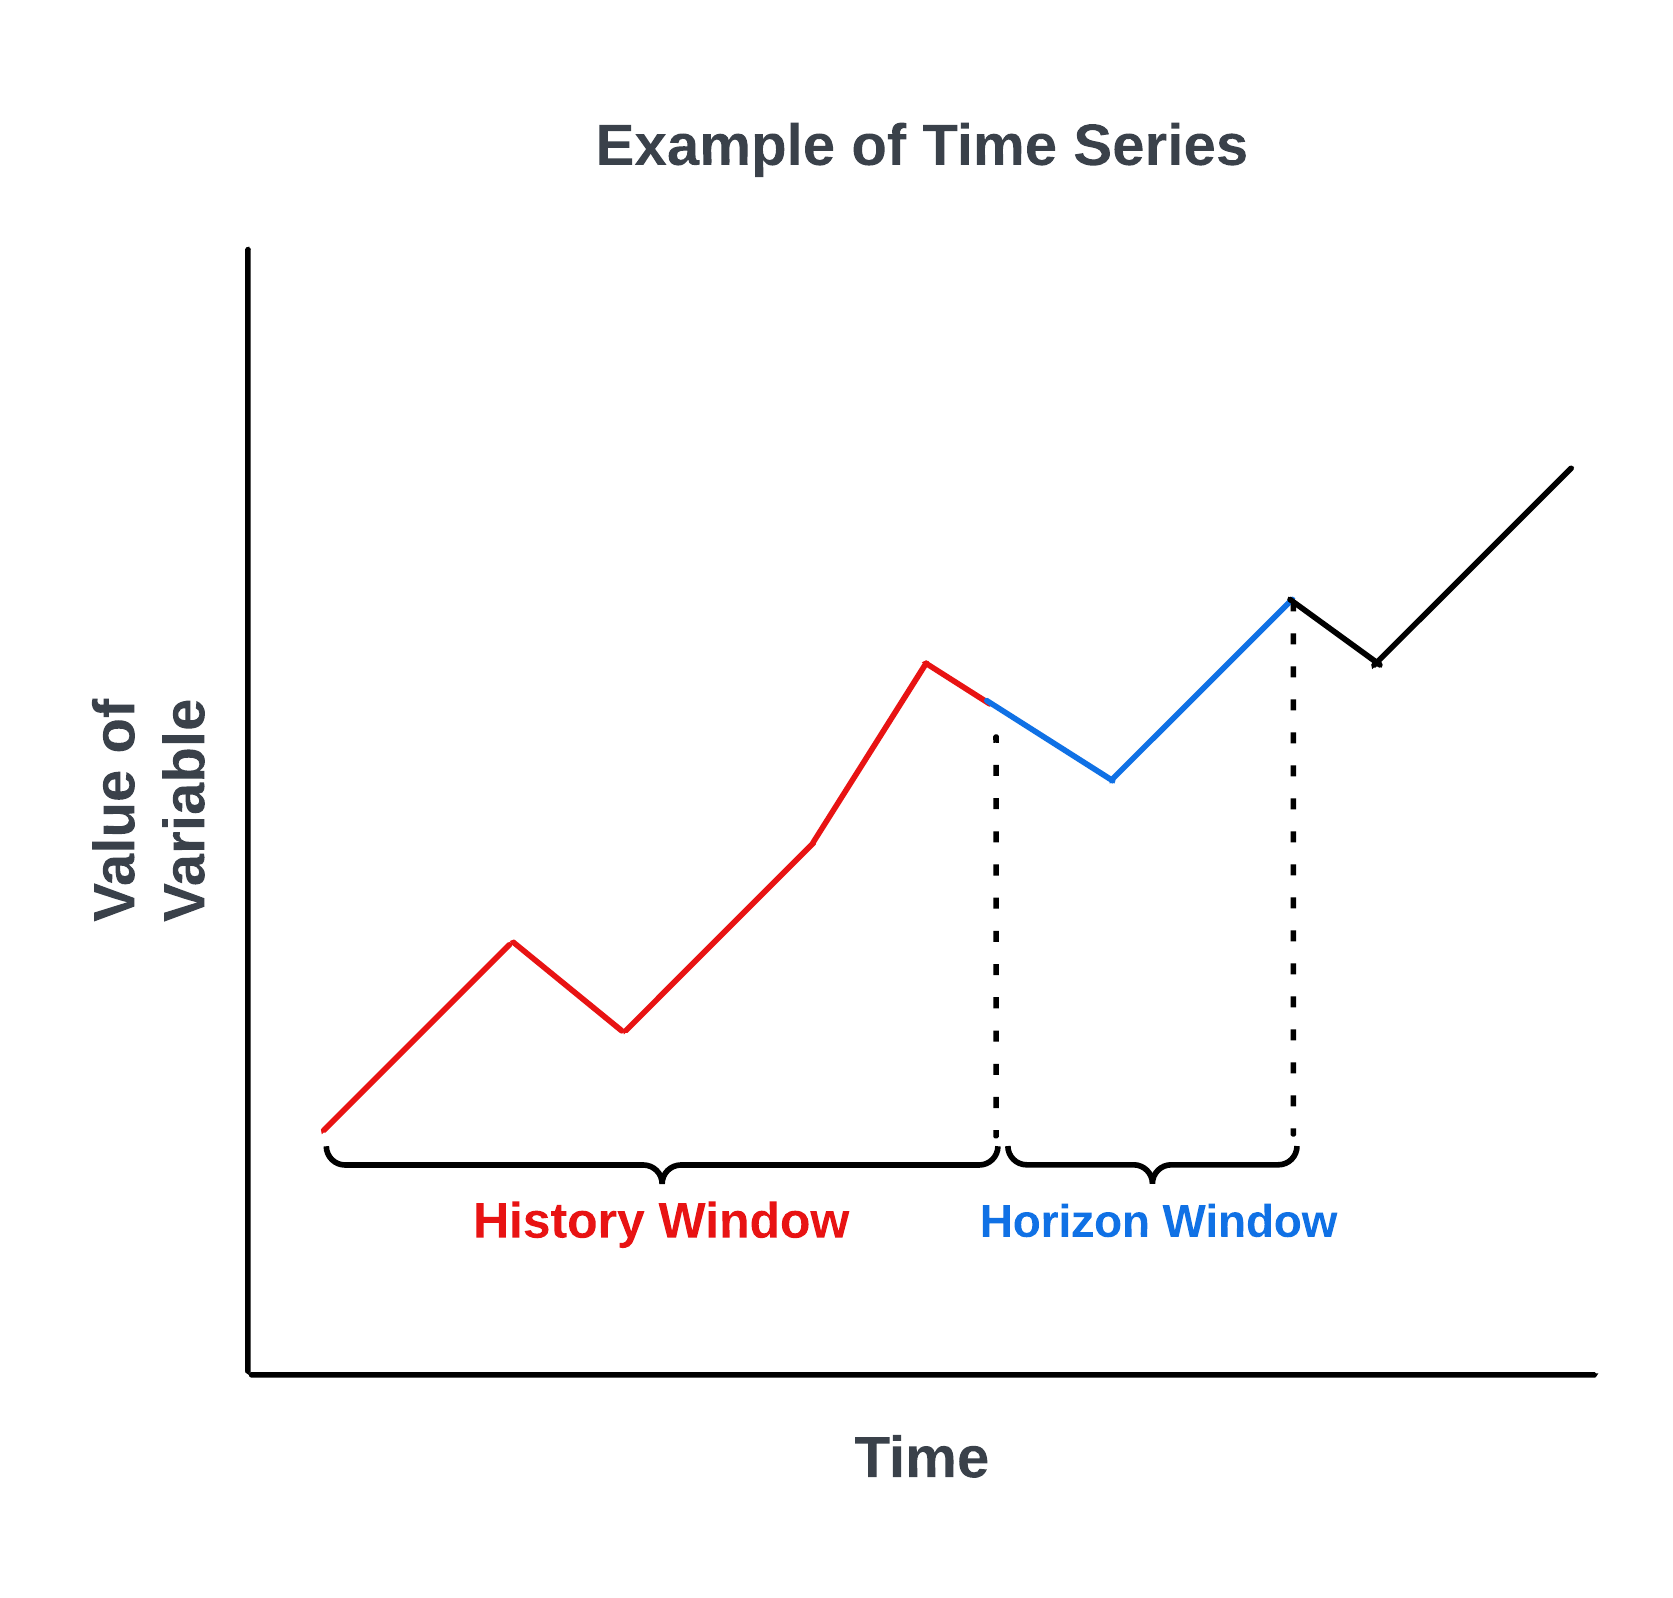
\includegraphics[scale=0.15]{History Horizon.png}
\centering
\caption{Graph showing how a history and horizon window can be constructed for a feature in time series data}
\label{fig:example_of_ts}
\end{figure}

There are many methods for identifying the optimal length of the horizon and history windows. Well studied methods such as the ACF (auto correlation function) or PACF (partial auto correlation function) \cite{10.2307/2958346} are useful for identifying temporal dependencies in the univariate case. The multivariate case is more complex as the target depends not only on previous values of itself, but previous values of other features. Still ACF provided a useful insight into the choices of history windows to consider. An ACF of <0.4 indicates that including values at the time lag does not contribute greatly to predicting the current value. An ACF >0.8 indicates that a particular lag is very relavant when predicting the current and future value of a metric.

Looking at figure \ref{fig:dl_acf} which shows the average ACF of the download throughput over the previous minute we observed that significant contributions to the prediction of current values falls off after 26 seconds. The red shaded region shows the standard deviation of the ACF observed over all traces. Intuitively this also suggests that for a horizon window of 5 seconds, 21 seconds would be an adequate maximum bound to consider for the history window. 

\begin{figure}[h]
\includegraphics[scale=0.5]{Images/Average_DL_bitrate_ACF.png}
\centering
\caption{This figure shows the average value of the auto correlation function for download throughput over all traces}
\label{fig:dl_acf}
\end{figure}

A selection of different combinations of horizon and history windows were considered to evaluate the impact each has on the throughput horizon predictions. The horizon window is more application dependent. The granularity of data available to us through G-NetTrack Pro is one second. In general more time sensitive applications such as web-conferencing would benefit a smaller horizon window. This incurs the cost of more computational power as the throughput prediction model must be run more frequently. Inversely, less time sensitive applications could use a longer horizon window. For throughput prediction, if the average horizon throughput is the main variable of interest then a longer horizon length may actually benefit predictions as the average will be calculated over a greater number of throughput predictions \cite{raca2019improving}.

\section{Selection of train/test Splits}
Typical train/test splits divide the dataset in a given ratio, usually 80:20 for train and test respectively. This is difficult to reproduce with this dataset as the dataset is not a single continuous time series but a collection of 135 distinct time series experiments. Train and test can be created by dividing the dataset based on the number of traces however, as seen in \ref{sec:distribution} the traces are of varying length making it difficult to split the dataset based on solo on the count. Another issue is that the training set must contain an adequate count of examples for all 3 classes, low, medium and high. As the classes are imbalanced, blindly partitioning the dataset based on traces may lead to situations where all examples of a single class ends up in either the training dataset or the testing dataset. This is especially the true for low throughput examples which have the least representation in the dataset. Both the baseline model and the multistage architectures must use the same train and test in order to be comparable. Failure to provide adequate examples of each class in the training data would result in the multistage models performing poorly. Instead, division of the traces was viewed an an optimisation problem. For each trace, the number of observations for each class of low, medium and high throughput was calculated. The number of observations of each class will vary based on the chosen horizon length and as such, different choices of horizon length will require a different train and test partition. The output of this process is as follows:
\begin{table}[!htb]
  \centering
  \caption{Example of Label Counting Output}
  \begin{tabular}{|c|c|c|c|}
    \hline
    Trace No. & Low Sequence Count & Medium Sequence Count & High Sequence Count \\
    \hline
    0 & 10 & 30 & 100 \\
    1 & 4 & 32 & 70\\
    2  & 0 & 60 & 130\\
    \hline
  \end{tabular}
\end{table}
The class counts per trace were then used to calculate a percentage of the total number of observations in each class over all traces contained within each trace. These percentages are then used partition the 135 traces in a given ratio (4:1 was used) in order to achieve the desired distribution of sequences in the train/test sets. Ideally the train set would include: \\
- 80\% of all low samples, 80\% of all medium samples and 80\% of all high samples \\
- Test would be the remainder i.e 20\% of low, medium and high \\

In practice it is difficult to find a split of traces that achieves the perfect ratio between low/medium/high for train and test. Instead a large number (10000) of potential splits are created and their class \% are measured. The split that is chosen is the train/test split with the lowest sum of differences between \% training low, medium, high, that is to say, train/test split chosen has the closest distribution to the desired distribution outlined above. The preprocessing code provides a summary of the distribution of the train/test split it finds. For example, most of the analysis in this paper focuses on a history window of 10 seconds and a horizon window of 5 seconds. The distribution of the train / test split for this selection is shown in table \ref{tab:train_test_dist}. 

\begin{table}[!htb]
  \centering
  \caption{Train/Test Class Distribution}
  \npdecimalsign{.}
  \nprounddigits{5}
  \begin{tabular}{|n{1}{4}|n{1}{4}|n{1}{4}|n{1}{4}|n{1}{4}|n{1}{4}|n{1}{4}|}
    \hline
    {train low} & {train medium} & {train high} & {test low} & {test medium} & {test high} & {distribution diff} \\
    \hline
	0.8646586591494055 & 0.8362963871178682 & 0.8373981034769589 & 0.1353413408505944 & 0.1637036128821317 & 0.162601896523041 & 0.0567245440630745\\
    \hline
  \end{tabular}
  \npnoround
  \label{tab:train_test_dist}
\end{table}

\section{Identifying Bounds for Mutlistage Model Classes}
\label{sec:bounds}
Two multistage approaches for modelling throughput prediction were considered in this paper. Each of the two architectures however share the same base models. Both multistage architectures proposed make use of a simple classifier that aims to predict a horizon throughput as one of 3 distinct situations, low throughput, medium throughput or high throughput. The choice to divide the problem based on the value of the download throughput comes from the fact that traces typically reported throughput above certain bounds (5Mbps, 1Mbps etc) far more often than below them. This imbalance leads to a single stage model frequently overestimating in low/medium throughput situations. Overestimating in these low or medium throughput scenarios leads to a noticeable decrease in the perceived quality of experience in applications such as video streaming \cite{raca2019improving} and is one of the main motivations of the multistage approach. 

The choice of the number of bounds (and subsequently models) and how to classify a given sequence of input data is arbitrary. For the purposes of this paper, dividing the data into one of three bounds sufficed. The sequences were divided by horizon download throughput into the three following ranges:

•Low:    $ mean[y] < 1Mbps$ \\
•Medium: $1Mpbs \leq mean[y] \leq 5Mpbs$ \\
•High:   $ mean[y] > 5Mbps$ \\

For forecasting, Lstm models are typically trained on x, y pairs where x is historic data of the predictor features over the past p seconds and y is the true value of the target variable of the next k seconds. The average download throughput of y was used to classify a given trace as an example of high, medium or low throughput.

The bounds 1Mbps and 5Mbps were chosen based on domain knowledge. Popular video streaming applications provide guidelines for the required download throughput for given video quality. As of the time of writing, 720p video requires 3Mbps on Netlfix whereas Youtube and Amazon Prime Video require at least 5Mbps of download throughput. While the adoption of AV1 hardware encoding may lower the required bitrate for HD video, use of the codec is still a while off mass market adoption and providers could choose to maintain the current bitrate while providing better quality source content.

\section{Feature Selection}
Feature selection is an important step in any machine learning problem. Good feature selection is known to improve loss, increase runtime performance and improve the understandability of predictions \cite{guyon2003introduction}.
Feature selection for multivariate time series is still an evolving field. The challenge is that the a selected feature set must capture the correlation between the target variable and predictors as well as between the target variable and lagged values of the predictors.

Feature selection is important for the analysis of multistage vs single stage throughput predictors explored this paper as it is an effective method in reducing the number of parameters of a given model. This is especially important when tight constraints are put on model size (in memory) and speed of inference, as is the case for models intended for mobile devices.

The number of feature included in the dataset is relatively small at 19 by current deep learning standards. This allows for methods such as exhaustive search to be viable, however hardware limitations prevented us from carrying out such an analysis due to time constraints. Geo-location data related to the serving cell tower was excluded from consideration. This data is currently not readily available on mobile devices and had to be gathered from a third party source \href{https://opencellid.org/}.

Firstly to explore the correlation between features. Fig \ref{fig:feature_correlation} shows the average correlation matrix over all traces. The features: RSRQ, RSSI, RSRP, NRxRSRP and NRxRSRQ are measured on a logarithmic scale and as such were transformed using the following formula before calculating the correlation matrix:
\begin{equation}
Y = exp(\left|X\right|)
\end{equation}
NetworkMode\_\{X\} is the one-hot-encoded transform of the NetworkMode feature, the same is true for State\_I and State\_DBefore performing this transform correlation between DL\_bitrate and these features was not observed. Understanding this matrix requires some careful thought. Firstly, this is a time series problem, DL\_bitrate will be used to predict itself. Knowing this, the observed strong correlation between DL\_bitrate and UL\_bitrate is misleading in regards to feature selection. This matrix suggests that including UL\_bitrate might actually be redundant. SNR and CQI are good candidates for inclusion in the optimal feature subset. RSRQ and NRxRSRP are also good candidates for inclusion. RSRQ has strong correlation with both CQI and SNR suggesting that one of either SNR or CQI could be also be dropped should constraints call for it. Geo-location data had no correlation with DL\_bitrate which is to be expected as the dataset was constructed from mobile devices in a relatively small geographic area. The NetworkMode variables were one-hot encoded and as such correlation is less applicable for these features. This matrix suggests that a good feature selection would include:

-DL\_bitrate \\
-SNR \\
-CQI \\
-NRxRSRP \\
-RSRQ \\

\newpage
\begin{figure}[h]
\includegraphics[scale=0.5]{Images/feature_correlation.png}
\centering
\caption{Correlation matrix showing the average correlation between features over all traces}
\label{fig:feature_correlation}
\end{figure}

Next permutation feature importance was considered. An Lstm was fit on all network related features, as well as location data for the mobile device. The Lstm used was the standard Lstm identfied in section \ref{sec:model_tuning} The metric we chose to compare the results of this test is the mean absolute percentage error (MAPE) given by the following formula: \\

\begin{equation}
MAPE = \frac{1}{n} \times \frac{\left|true-predicted\right|}{true} \times 100
\end{equation}
where $n$ is the number of observations in the test set.

The procedure for permutation feature importance is as follows:

- Given a target variable $Y$, with predictor variables $X=\{X_1,X_2,X_3,...X_n\}$ \\
- Create a train/test split of the dataset \\
- Fit a model on the training data using all features in $X$ \\
- Compute the loss of the model on the test set to use as a baseline \\
- Randomly shuffle the values of one feature $X_k$ in the test set and compute the loss with just this feature's values shuffled. Do this $\forall X_k \in X$. \\
- Compared the performance of the model on the test set with the performance of the model on each test set with a shuffled feature \\
- Rank the features based on the difference in performance \\
- Use this ranked list to identify possible features to eliminate \\

The results of this analysis can be seen in figure \ref{fig:feature_importance}. In this case the model relied heavily on the NetworkMode feature. RSRQ was once again important in improving prediction performance. 
\newpage
\begin{figure}[h]
\includegraphics[scale=0.5]{Images/feature_importance.png}
\centering
\caption{Bar Chart showing Difference in Model Performance with Permuted Feature Column.}
\label{fig:feature_importance}
\end{figure}


\section{Imputation \& Scaling}
In section \ref{sec:missingness} we observed that the majority of missing values can be categorised as MNAR (missing not at random). 
\chapter{Design}
The focus of this paper is to explore the differences between a single model and a multistage architecture for throughput prediction in wireless networks. The choice of machine learning or deep learning model must therefore be consistent across all models considered to avoid confusing the issue with that of comparing one ML (machine learning) or DL (deep learning) method of regression with another. Lstm (long short-term memory) networks are recognised as effective models for time series forecasting \cite{8614252}, with deep learning models in general performing well in networking related tasks \cite{8666641}. As such any individual model considered in this paper is some form of Lstm deep network. Initial comparisons of multistage vs a single model ensure that all Lstm models have the same hyperparameters. That is to say, all models have the same number of nodes, layers, the same dropout chance, activation function, optimizer, etc. The only difference between the individual models considered will be that the classifier model has a different output layer to the traditional regression models as it aims to predict the class of the input sequence as opposed to the DL\_bitrate horizon. In total there are 5 individual Lstm models that had to be trained with brief description given in \ref{tab:brief_models}

\begin{table}[!htb]
  \centering
  \caption{Lstm Deep Models Used}
  \begin{tabular}{|c|c|c|}
  \hline
    {Model} & {Training Data} & {Outputs} \\
    \hline
	Baseline & All TP examples & DL\_bitrate prediction horizon \\
	\hline
	Low & Only Low TP examples & DL\_bitrate prediction horizon \\
	\hline
	Medium & Only Medium TP examples & DL\_bitrate prediction horizon \\
	\hline
	High & Only High TP examples & DL\_bitrate prediction horizon \\
	\hline
	Classifier & All labelled TP examples & Class probability table \\
  \hline
  \end{tabular}
  \label{tab:brief_models}
\end{table}


In \ref{CONSTRAINTS HEREHERHEHREHR} the number of parameters of the Lstm models were altered in various ways in order to achieve memory size parity between the single baseline throughput predictor and the multistage predictors. This is an important point to explore as adoption of a multistage approach vs a single model on mobile devices will require that both methods have comparable performance on hardware. A multistage approach could only be considered more optimal if the required memory and inference time were comparable. By design a multistage approach will be bigger than a single model, as such the total number of parameters of both approaches should be equalised for further comparison.

\section{Model Tuning}
\label{sec:model_tuning}
A hyperparameter is a parameter whose value is set before the learning process begins. In machine learning, a hyperparameter is a configuration variable that is used to control the training process, as opposed to the parameters of the model such as weights and biases, which are learned from the data. For Lstm deep models there are a number of hyperparameters than can be altered by the user, a few of note are:

- Choice of optimiser\\
- Learning rate \\
- Number of hidden nodes \\
- Number of layers \\
- Inclusion of dropout layers \\
- Dropout chance

Hyperparameter tuning is the practice of optimising the hyperparameters of a model in order to achieve better model performance. The impact of hyperparameters is wide reaching. The choice of hyperparameters not only affects the predictive performance of the model and model size, but also impacts less obvious metrics such as inference latency \cite{10.1145/3506695}. For models intended for low power devices such as mobile devices and IoT (internet of things) devices, hyperparameter tuning is even more important, as it can influence the battery consumption of the device \cite{10.1145/3506695}. The issue is with hyperparameter tuning is that the choice of hyperparameters leads to an infinite set of possible models. There are many methods for tuning deep learning models. As the models were implemented in Tensorflow, we made use of KerasTuner \cite{omalley2019kerastuner}, a tuning framework that allows for a low code solution to this issue. Random search was used to explore the possible set of combinations of hyperparameters as it is known to perform better than similar tools such as grid search \cite{bergstra2012random}. 

It must be noted that due to hardware and time limitations, only 10 such combinations of hyperparameters were considered for each model. The model was trained on each set of hyperparameters 3 times, in an attempt to account for different initialisation states leading to differences in model performance. This process was by no means extensive and given more time and computational power, a larger set of hyperparameters should be considered.

\section{Multistage One}
\begin{figure}[h]
\centering
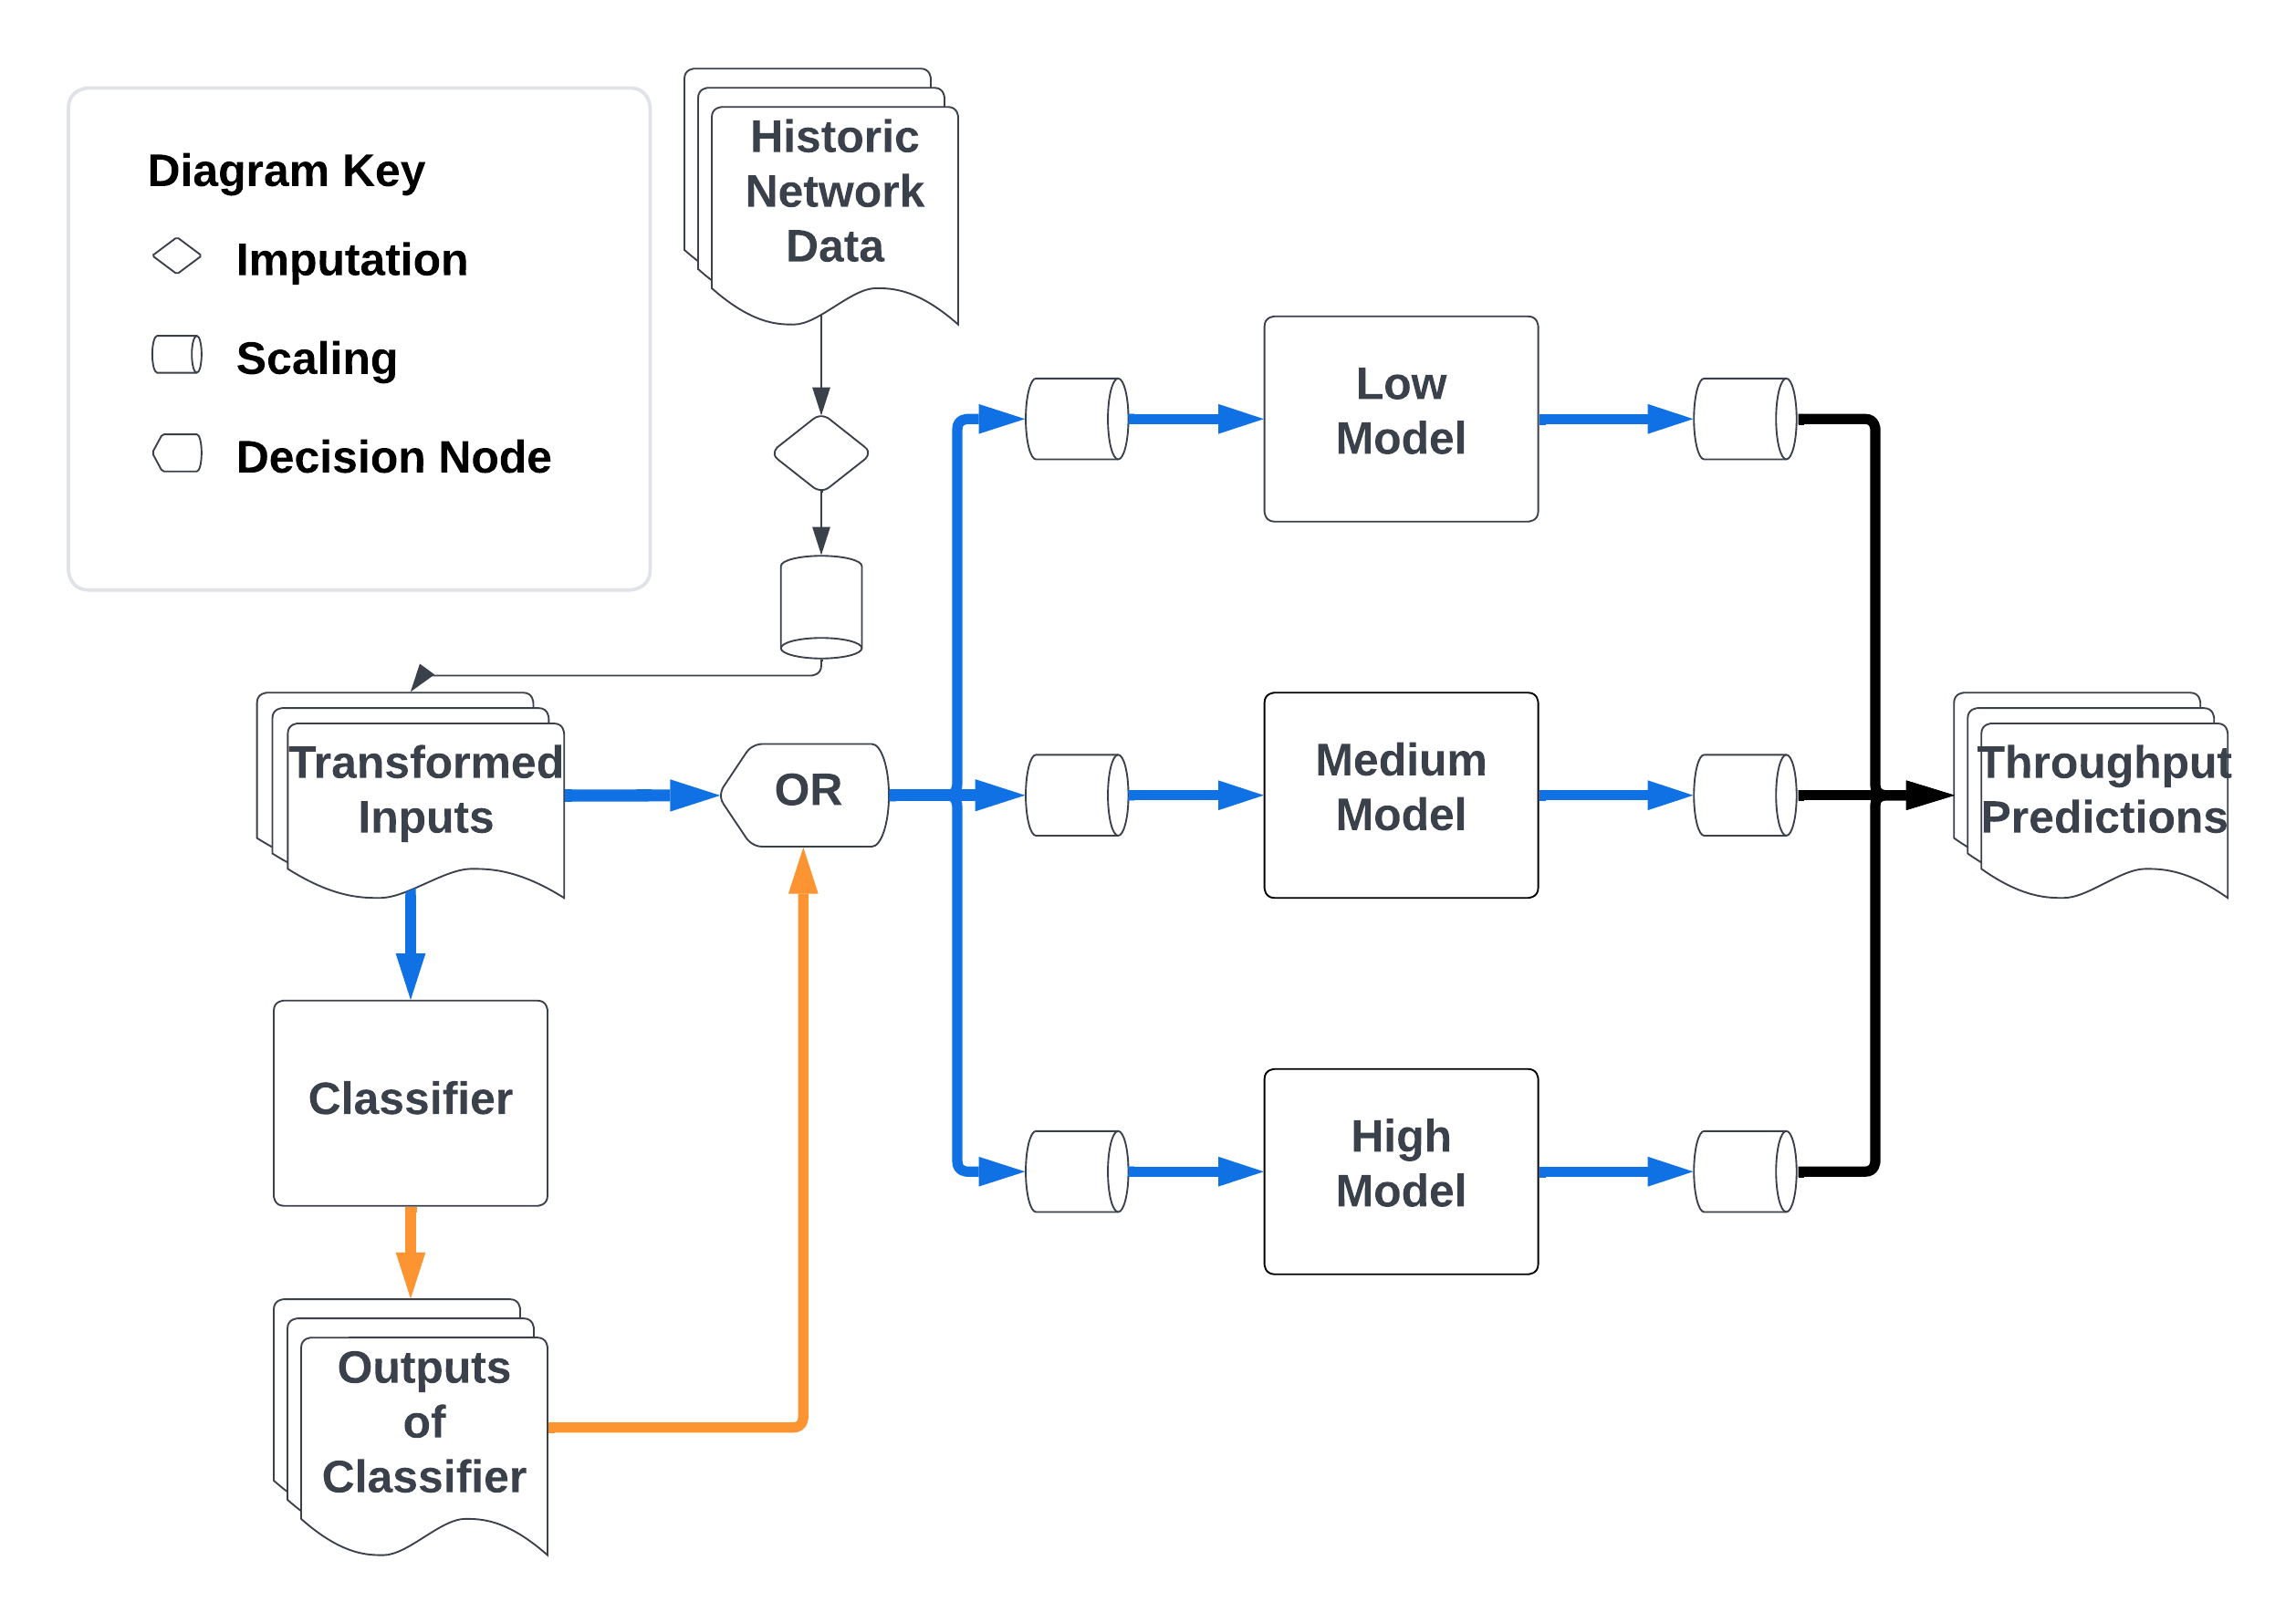
\includegraphics[scale=0.15]{Multistage One.png}
\label{fig:multistage_one}
\caption{Multistage One model.}
\end{figure}

The multistage throughput predictor herein referred to by "multistage one" uses a classifier to predict the most likely throughput class of the horizon for a given history sequence. As previously discussed, three classes are considered, high, medium and low, which describe the group the horizon throughput based on sub-ranges. Refer back to section \ref{sec:bounds} for a detailed description on the construction of these classes from the dataset. Based on the classifier's decision, the input is passed to one of the three regression models, each trained exclusively on examples of sequences of their respective class. As only one model is chosen, performance of this architecture is heavily dependent on correct classification of the horizon throughput scenario by the classifier. Misclassification of an input sequence will lead to the wrong regression model being chosen for throughput prediction negating the advantage of the multistage approach vs a single model entirely. Figure \ref{fig:multistage_one} shows the higher level design of the multistage one model.

\section{Multistage All}
\begin{figure}[h]
\centering
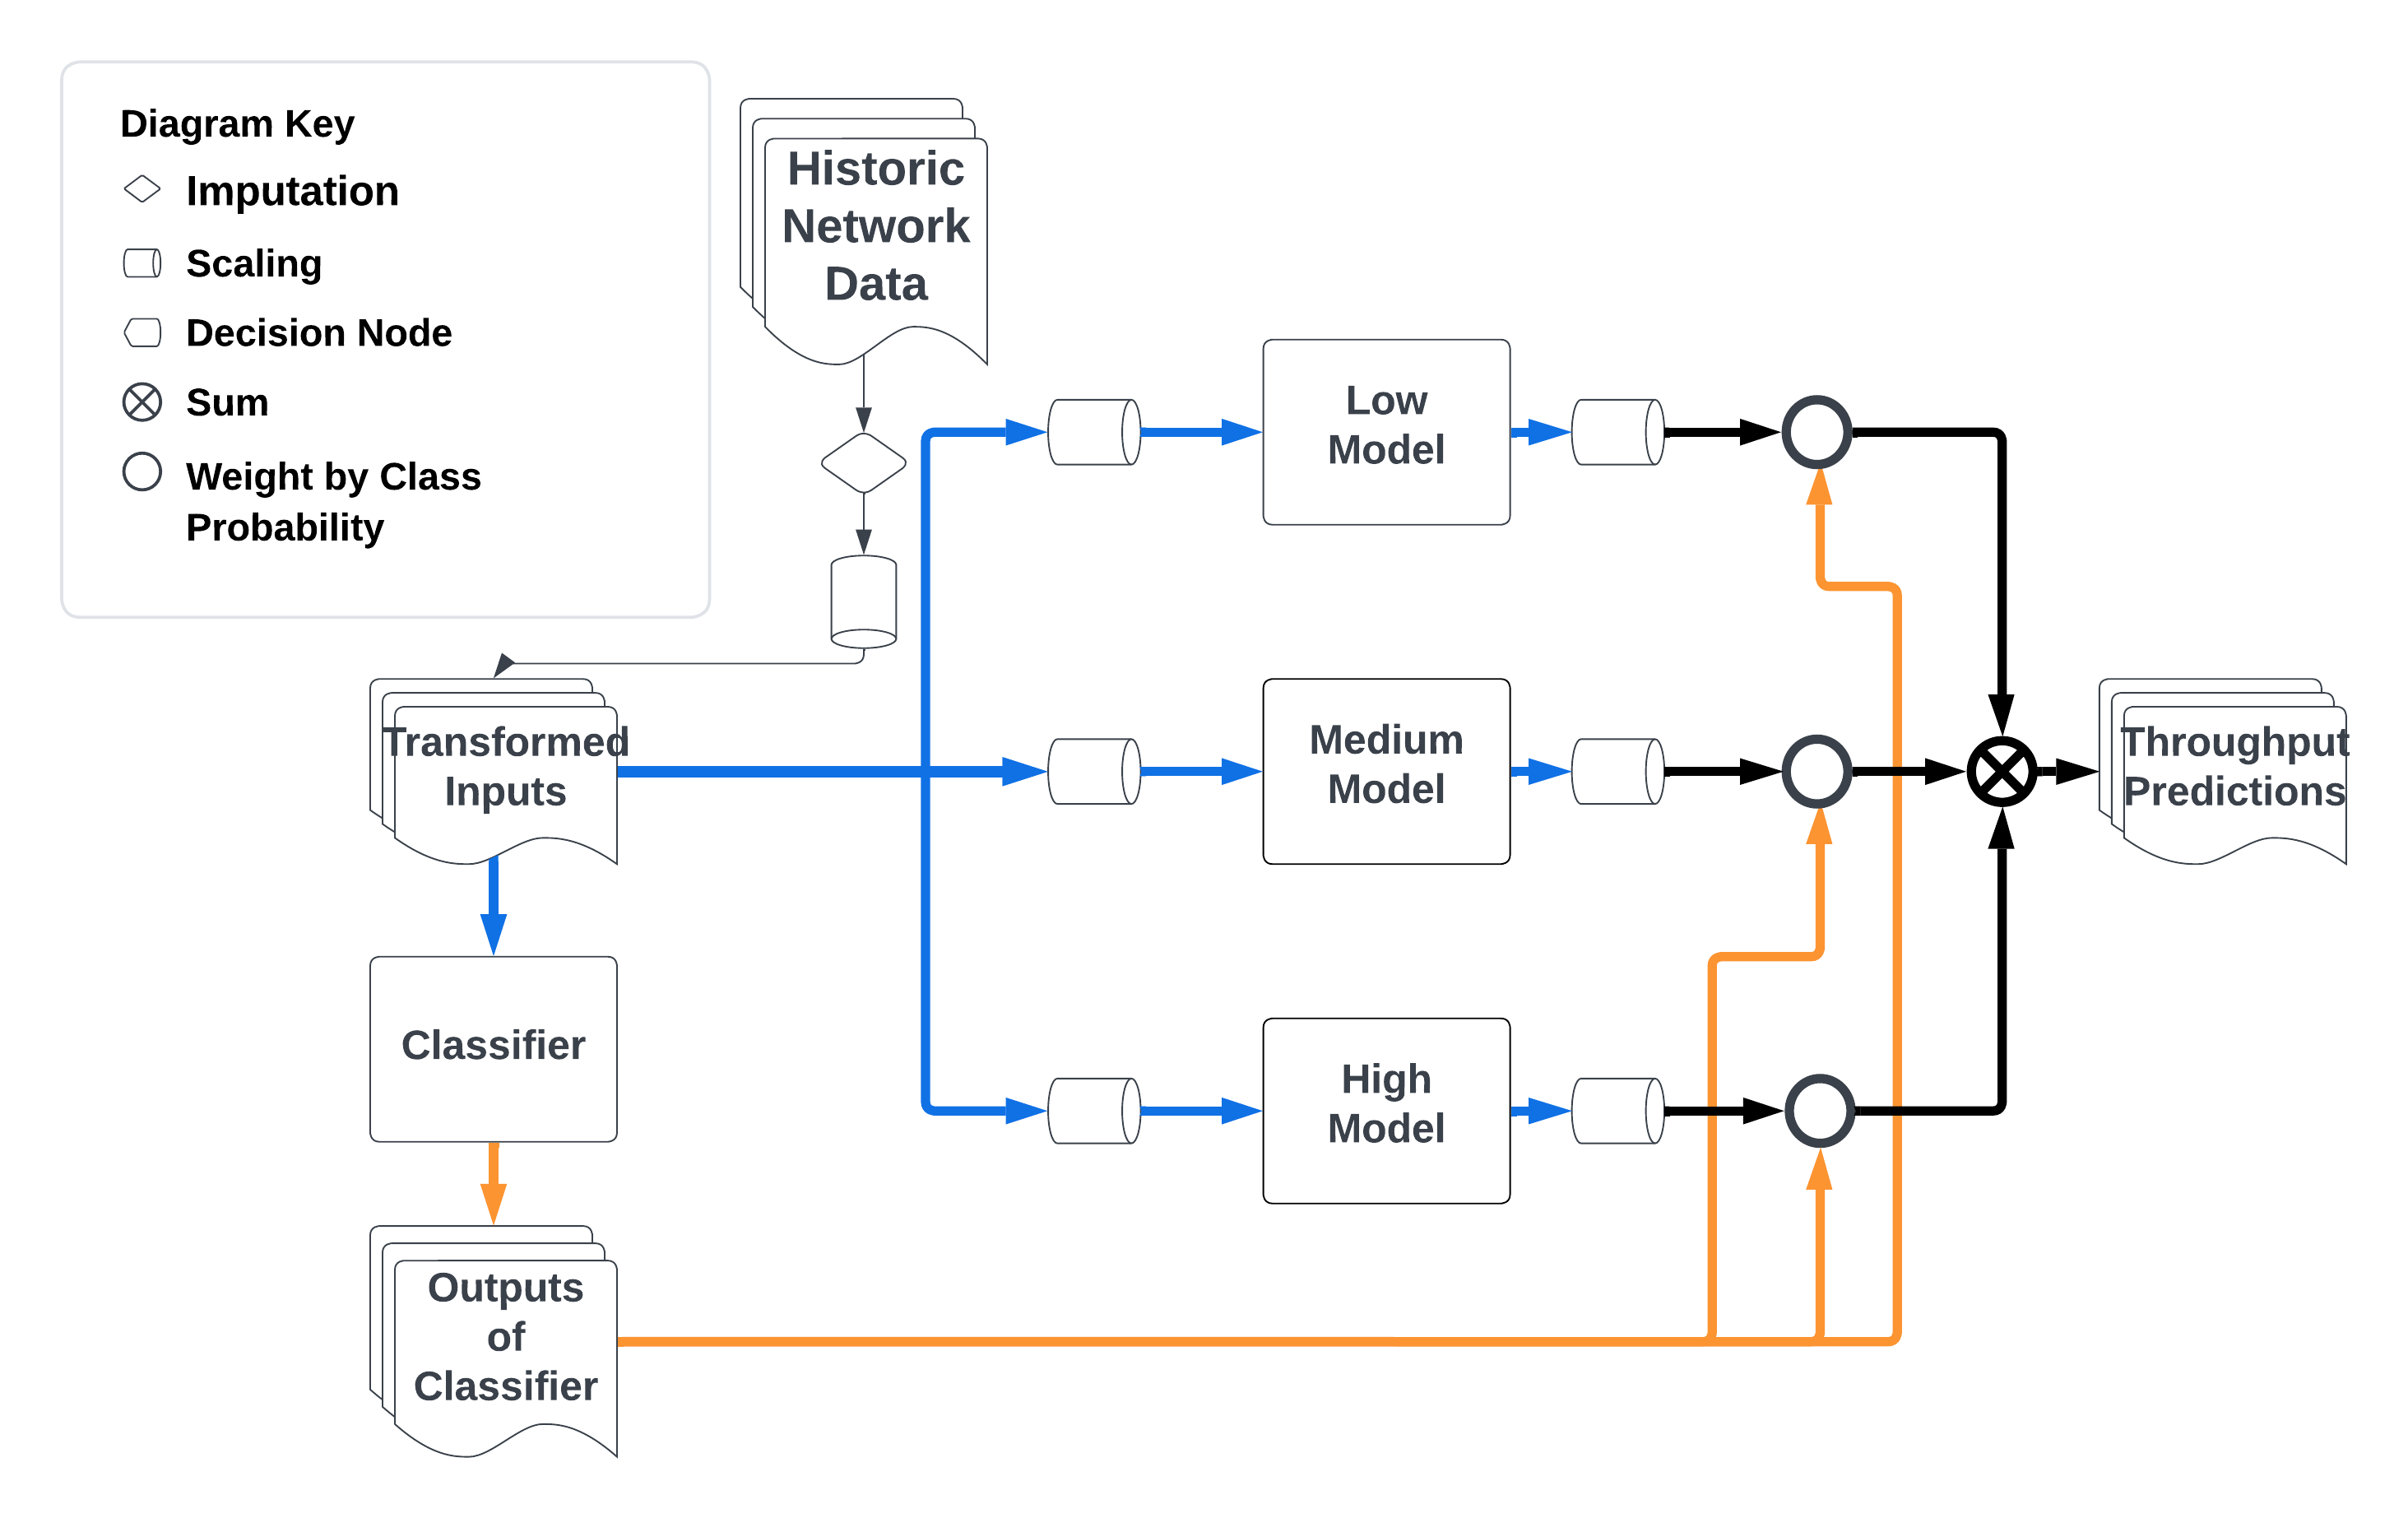
\includegraphics[scale=0.15]{Multistage All.png}
\label{fig:multistage_all}
\caption{Multistage All model.}
\end{figure}

The multistage throughput predictor herein referred to by "multistage all" uses a classifier to predict the probability of each of the classes of the horizon for a given history sequence. Unlike the multistage one model, the input sequence is then passed to all three regression models. The outputs of the regression models are then weighted by the class probability vector from the classifier and summed to create the final prediction. This is essentially an ensemble model. Ensemble models are known to perform better than using a single model \cite{https://doi.org/10.1002/widm.1249}. This model should perform better in situations where the classifier made less definite predictions on the input sequence's class. In theory, sequences on the border of two classes are better accommodated for by this model compared to the multistage one model. Figure \ref{fig:multistage_all} shows the higher level design of the multistage all model.

\section{Testing Framework}
To properly test the multistage approaches we first had to prove the rational to construct the multistage models based on the division of the range of DL\_bitrate. To do this we first test the individual regression models on their respective test sets and compare this to the baseline model's performance on the same test set. This shows that a model trained on a restricted range will be better at predicting values within that range. We then compare the performance of the multistage one, multistage all and baseline model on the complete test set. The complete test set is the baseline model's test set or the sum of the low, medium and high model's test sets. This shows actual performance of the multistage approaches as test sequences will be passed through the entire multistage frameworks for inference. We then considered the multistage models performance on the low and medium test sets in particular vs the baselines performance to identify in where difference in overall performance stemmed from. Results were calculated on the actual scale of the data in order to improve the understandability.

The following metrics were considered in the comparison:

- Mean Squared Error (MSE)\\
- Mean Absolute Error (MAE)\\
- Mean Absolute Percent Error (MAPE)\\
- Residual boxplots \\ 
- Absolute Percent Error boxplots \\

Relative error metrics such as MAPE are the most important in this application as they take into account that errors in lower throughput situations are more critical than errors in high throughput situations. I.e. A difference of 2Mbps in the prediction vs the true throughput when the predicted value is 152Mbps and the true value is 150Mbps is far less important than a difference in 2Mbps when the predicted throughput is 3Mbps and the true throughput is 1Mbps.

All tests were run on the same system. Specs are as follows: \\

- Cpu : Ryzen 5 1600 (6 cores / 12 threads) \@ 3.6Ghz
- GPU : Gtx 1050ti
- Ram : 32GB cl 3200 
\chapter{Testing}
Testing methodology, baseline model, metrics etc.
\chapter{Conclusions}
The usefulness of multistage deep models in throughput prediction has been shown in this paper, with multistage models providing a noticable increase in relativistic measures of model performance such as percentage based errors. The multistage one architecture proposed in this paper proved to be the best of the 3 methods considered for throughput prediction in wireless cellular networks. The variability in cellular network channels still poses a challenge for throughput prediction algorithms with much room left for improvement. Now that the multistage approach has been proven viable for consideration in both non size-constricted and size-constricted deployments, the possibility exists to explore new multistage architectures to tackle the problem of wireless throughput prediction. More work still needs to be done on building and testing these models for deployment on mobile devices, as well optimisation of the sub-models used to construct a multistage approach.
\end{document}